\documentclass[border=2pt]{standalone}
\usepackage[dvipsnames,svgnames,x11names]{xcolor}
\usepackage{tikz}
\usetikzlibrary{arrows.meta,backgrounds,fit}
\begin{document}
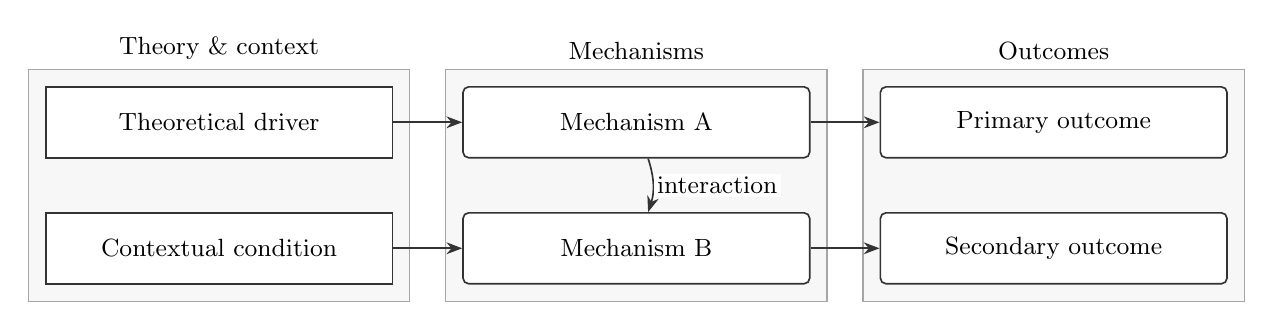
\begin{tikzpicture}[font=\small,>=Stealth,x=53.0mm,y=16.0mm]
\node[rectangle,fill=white,draw=black!80,text=black,line width=0.6pt,minimum height=9mm,inner xsep=7pt,inner ysep=4.5pt,align=center,text width=39.1mm,execute at begin node={\hyphenpenalty=10000\relax}] (t1) at (0,0) {Theoretical driver};
\node[rectangle,fill=white,draw=black!80,text=black,line width=0.6pt,minimum height=9mm,inner xsep=7pt,inner ysep=4.5pt,align=center,text width=39.1mm,execute at begin node={\hyphenpenalty=10000\relax}] (t2) at (0,-1) {Contextual condition};
\node[rectangle,rounded corners=2pt,fill=white,draw=black!80,text=black,line width=0.6pt,minimum height=9mm,inner xsep=7pt,inner ysep=4.5pt,align=center,text width=39.1mm,execute at begin node={\hyphenpenalty=10000\relax}] (m1) at (1,0) {Mechanism A};
\node[rectangle,rounded corners=2pt,fill=white,draw=black!80,text=black,line width=0.6pt,minimum height=9mm,inner xsep=7pt,inner ysep=4.5pt,align=center,text width=39.1mm,execute at begin node={\hyphenpenalty=10000\relax}] (m2) at (1,-1) {Mechanism B};
\node[rectangle,rounded corners=2pt,fill=white,draw=black!80,text=black,line width=0.6pt,minimum height=9mm,inner xsep=7pt,inner ysep=4.5pt,align=center,text width=39.1mm,execute at begin node={\hyphenpenalty=10000\relax}] (o1) at (2,0) {Primary outcome};
\node[rectangle,rounded corners=2pt,fill=white,draw=black!80,text=black,line width=0.6pt,minimum height=9mm,inner xsep=7pt,inner ysep=4.5pt,align=center,text width=39.1mm,execute at begin node={\hyphenpenalty=10000\relax}] (o2) at (2,-1) {Secondary outcome};
\begin{scope}[on background layer]
\node[fit=(t1)(t2),inner sep=6pt,fill=black!3,draw=black!35,line width=0.45pt,label={[font=\small]above:{Theory \& context}}] (drivers) {};
\node[fit=(m1)(m2),inner sep=6pt,fill=black!3,draw=black!35,line width=0.45pt,label={[font=\small]above:{Mechanisms}}] (mechanisms) {};
\node[fit=(o1)(o2),inner sep=6pt,fill=black!3,draw=black!35,line width=0.45pt,label={[font=\small]above:{Outcomes}}] (outcomes) {};
\end{scope}
\draw[->,draw=black!80,line width=0.6pt] (t1) -- (m1);
\draw[->,draw=black!80,line width=0.6pt] (t2) -- (m2);
\draw[->,draw=black!80,line width=0.6pt] (m1) -- (o1);
\draw[->,draw=black!80,line width=0.6pt] (m2) -- (o2);
\draw[->,draw=black!80,line width=0.6pt] (m1) to[bend left=18] node[pos=0.5,right,fill=white,inner sep=1.2pt] {interaction} (m2);
\end{tikzpicture}
\end{document}
